\chapter{Risks}
There are a number of risks to this project, as with all software development projects. A Risk Breakdown Structure (RBS) is a method defined in the PMBOK guide \cite{pmbok2013} of breaking down and categorising risks in a project to enumerate the risks. This ensures everyone is aware of what they are, so that they can best be avoided, mitigated, or otherwise dealt with. PRINCE2 \cite{prince2} further describes these processes in-depth, which our team will incorporate to ensure the highest chance of success for the project.

% Removed the section headings because there is not much content here at the moment
%\section{Risk Breakdown Structure}

%\section{Failure Modes and Effects Analysis}

After carefully analysing the project objectives and resources needed for their completion, the team devised a list of risks associated with the project using the RBS method. Next, each risk was evaluated in terms of their severity, occurrence, and detectability, according to the Failure Modes and Effects Analysis (FMEA). This analysis is invaluable in analysing individual systems' possible flaws and failures, and what risks they pose. Additionally, it provides a quantitative score of overall risk which can be compared to the risk after mitigations are applied, allowing for informed decision-making regarding prioritisation of countermeasures. The effects of our RBS and FMEA analyses are presented in table \ref{tab:fmea}.

\begin{table}
    \centering
    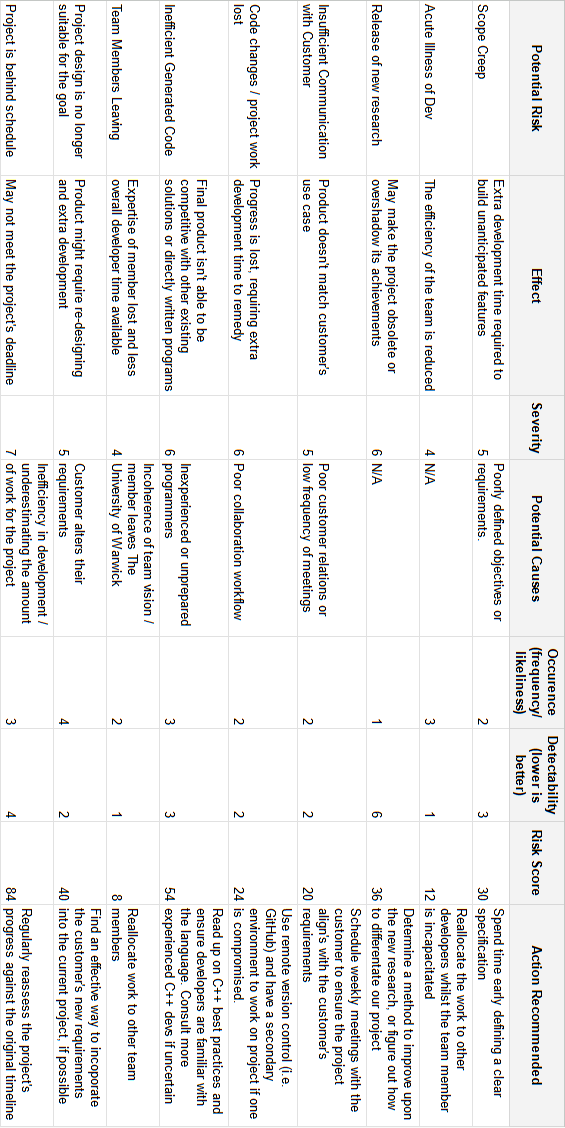
\includegraphics[width=10cm]{thesis/diagrams/risks.png}
    \caption{Failure Modes and Effects Analysis}
    \label{tab:fmea}
\end{table}
